\documentclass[tikz,border=5pt]{standalone}
\usepackage{tikz}
\usetikzlibrary{arrows.meta, calc}
\usetikzlibrary{decorations.markings, arrows}
\usetikzlibrary{decorations.shapes}
\usetikzlibrary{decorations.pathreplacing}

% --- Define Colors ---
\definecolor{myblue}{RGB}{175, 204, 233}
\definecolor{mygreen}{RGB}{125,208,163}

\tikzstyle{blue} = [draw=black,outer sep=0, inner sep=5,
    minimum width=1cm, minimum height=1cm, line width=1,
    top color=myblue, bottom color=myblue, font=\Large, align=center]
\tikzstyle{green} = [draw=black,outer sep=0,inner sep=5,
    minimum width=1cm, minimum height=1cm, line width=1,
    top color=mygreen, bottom color=mygreen, font=\Large, align=center]


\tikzstyle{square} = [draw,outer sep=5,inner sep=3,minimum size=10,
    line width=0, very thick, draw=black!100,
    top color=white,bottom color=white, font=\Huge]
    
\tikzstyle{square2} = [draw,outer sep=5,inner sep=3,minimum size=10,
    line width=0, very thick, draw=black!100,
    top color=white,bottom color=white, font=\Large]
    
\tikzstyle{square3} = [draw=none,outer sep=5,inner sep=3,minimum size=10,
    line width=0, color=red!80!black,
    top color=white,bottom color=white, font=\Large]


\begin{document}

% ==================================================================
% FIGURE : REDUCTIONS
% ==================================================================
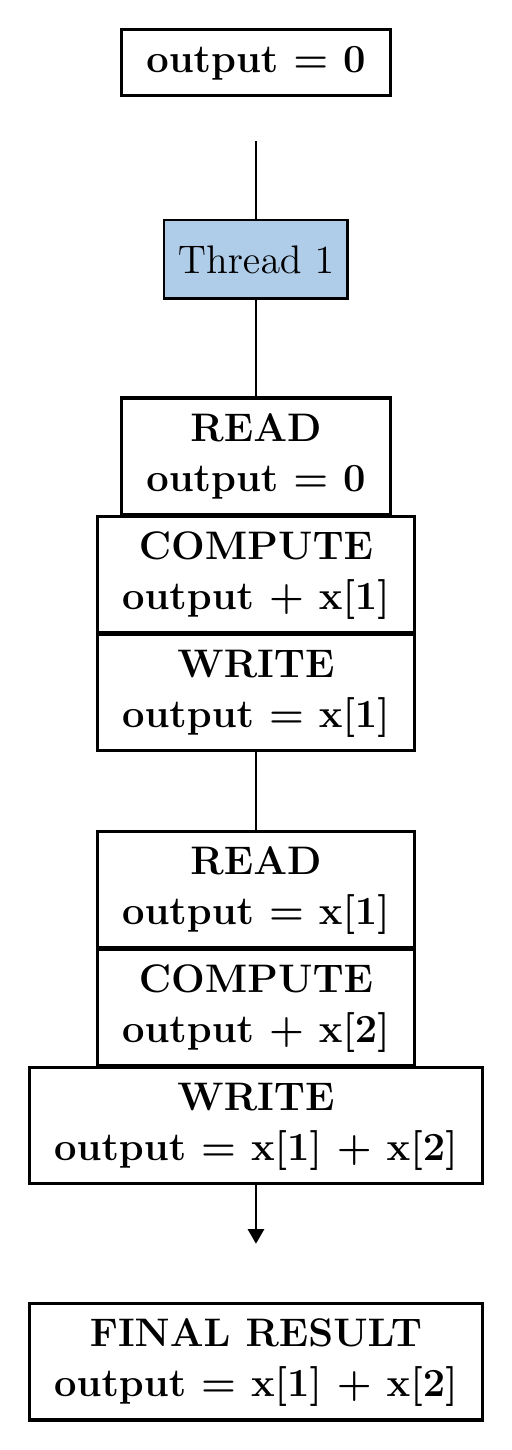
\begin{tikzpicture}



\node[square2] at (-6.5,7.5) {\textbf{\begin{tabular}{c} output = 0 \end{tabular}}};;



\draw[-triangle 60]  (-6.5,6.5) -- node[pos=1, anchor=west] {\textbf{\begin{tabular}{c} \end{tabular}}}(-6.5,-7.5);


%%% threads
\node[blue] (t2) at (-6.5,5) {Thread 1};


\node[square2] at (-6.5,2.5) {\textbf{\begin{tabular}{c} READ \\ output = 0 \end{tabular}}};
\node[square2] at (-6.5,1) {\textbf{\begin{tabular}{c} COMPUTE \\ output + x[1] \end{tabular}}};
\node[square2] at (-6.5,-0.5) {\textbf{\begin{tabular}{c} WRITE \\ output = x[1] \end{tabular}}};

\node[square2] at (-6.5,-3) {\textbf{\begin{tabular}{c} READ \\ output = x[1] \end{tabular}}};

\node[square2] at (-6.5,-4.5) {\textbf{\begin{tabular}{c} COMPUTE \\ output + x[2] \end{tabular}}};
\node[square2] at (-6.5,-6) {\textbf{\begin{tabular}{c} WRITE \\ output = x[1] + x[2] \end{tabular}}};



\node[square2] at (-6.5,-9) {\textbf{\begin{tabular}{c} FINAL RESULT \\ output = x[1] + x[2] \end{tabular}}};





\end{tikzpicture}

\end{document}
